\section{Random Number Generators}
\label{section:RNGs}

% This section was authored by Ralf Schlatterbeck (Ralf Schlatterbeck <rsc@runtux.com>)

\epigraph{``The generation of random numbers is too important to be left to chance.''}{Robert R. Coveyou}


\begin{figure}[h]
  \centering
  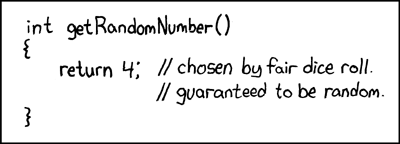
\includegraphics[width=0.4\textwidth]{img/random_number.png}
  \caption{xkcd, source: \url{https://imgs.xkcd.com/comics/random_number.png}, license: CC-BY-NC}
  \label{fig:dilbertRNG}
\end{figure}



A good source of random numbers is essential for many crypto
operations. The key feature of a good random number generator is the
non-predictability of the generated numbers. This means that hardware
support for generating entropy is essential.


Hardware random number generators in operating systems or standalone
components collect entropy from various random events mostly by using
the (low bits of the) time an event occurs as an entropy source. The
entropy is merged into an entropy pool and in some implementations there
is some bookkeeping about the number of random bits available.

\subsection{When random number generators fail}

Random number generators can fail -- returning predictable non-random
numbers -- if not enough entropy is available when random numbers should
be generated.

This typically occurs for embedded devices and virtual machines.
Embedded devices lack some entropy sources other devices have, e.g.:

\begin{itemize*}
  \item No persistent clock, so boot-time is not contributing to the
    initial RNG state
  \item No hard-disk: No entropy from hard-disk timing, no way to store
    entropy between reboots
\end{itemize*}

Virtual machines emulate some hardware components so that the
generated entropy is over-estimated. The most critical component that
has been shown to return wrong results in an emulated environment is the
timing source~\cite{Eng11,POL11}.

Typically the most vulnerable time where low-entropy situations occur is
shortly after a reboot. Unfortunately many operating system installers
create cryptographic keys shortly after a reboot~\cite{HDWH12}.

Another problem is that OpenSSL seeds its internal random generator only
seldomly from the hardware random number generator of the operating
system. This can lead to situations where a daemon that is started at a
time when entropy is low keeps this low-entropy situation for hours
leading to predictable session keys~\cite{HDWH12}.

For systems where -- during the lifetime of the keys -- it is expected
that low-entropy situations occur, RSA keys should be preferred over DSA
keys: For DSA, if there is ever insufficient entropy at the time keys
are used for signing this may lead to repeated ephemeral keys. An
attacker who can guess an ephemeral private key used in such a signature
can compromise the DSA secret key.
For RSA this can lead to discovery of encrypted plaintext or forged
signatures but not to the compromise of the secret key~\cite{HDWH12}.
